\chapter{Non-SD Contributions}\label{section:star_nonSD}
Events, in which  forward proton and reconstructed TOF
vertex are the result of the same $pp$ interaction, may originate from \ac{ND}, \ac{DD}, \ac{SD}, and \ac{CD} processes.  Their relative contributions must be estimated from MC models and are therefore model dependent. Tracks reconstructed in \ac{RP}s  %which are modeled in the~\ac{MC} simulations are only coming from:
may also be:
\begin{itemize}
	\item forward protons produced in the \ac{SD}, \ac{CD} or \ac{DD} diffractive systems or from \ac{ND} events,
	\item secondary particles from showering initiated 
	by interaction of forward protons with beam-line elements. This contribution is equal to approximately $2\%$.
\end{itemize}

Figure~\ref{fig:nonSDxit} shows the uncorrected $\xi$ and $t$ distributions in data compared to various \ac{MC} models: PYTHIA~8 A2 (MBR), PYTHIA~8 A2 (MBR-tuned) and EPOS. The \ac{MC} distributions are split into \ac{SD}, \ac{ND}, \ac{DD} and \ac{CD} components. For EPOS, SD$^\prime$ is separated from the ND events. Additionally, the accidental background is also shown. PYTHIA~8 A2 (MBR-tuned) predictions agree much better with the data than PYTHIA~8 A2 (MBR)  and result also in a suppression of non-SD events. EPOS describes data better than PYTHIA~8 but shows a dominant contribution of SD$^\prime$ events. All MCs predict significant \ac{DD} and \ac{ND} background at large $\xi$, thereby  the analysis was limited to $\xi < 0.2$. 

 \Cref{fig:nonSDnsel,fig:nonSDpt,fig:nonSDera} show the uncorrected distributions of variables used in the later analysis: $n_{\mathrm{sel}}$, $p_{\mathrm T}$ an $\bar{\eta}$. The  contributions from non-SD (except  EPOS-SD$^\prime$) interactions differ a bit between each other, i.e. EPOS predicts significantly larger CD contribution, whereas DD and ND are suppressed in PYTHIA~8 A2 (MBR-tuned).  PYTHIA~8~A2~(MBR) is used as the default model  of non-SD contribution subtracted from the data with systematic uncertainty $\pm50\%$, which covers all differences between the~models except EPOS-SD$^\prime$.  In this analysis EPOS-SD$^\prime$ is   considered as an~alternative to PYTHIA~8 SD model of events with forward proton in the final state,  where one of the proton remnants hadronizes back to a~single proton (non-diffrative process), while in  PYTHIA~8 the~initial proton stays intact (diffractive process). As a~consequence, results  are compared  with the~sum of SD and SD$^\prime$ procesess for EPOS model.   %Moreover, SD' in EPOS was not subtracted but used separately for comparisons.

\thispagestyle{empty}
\begin{figure}[h!]
	%\vspace{-0.5cm}
	\centering
	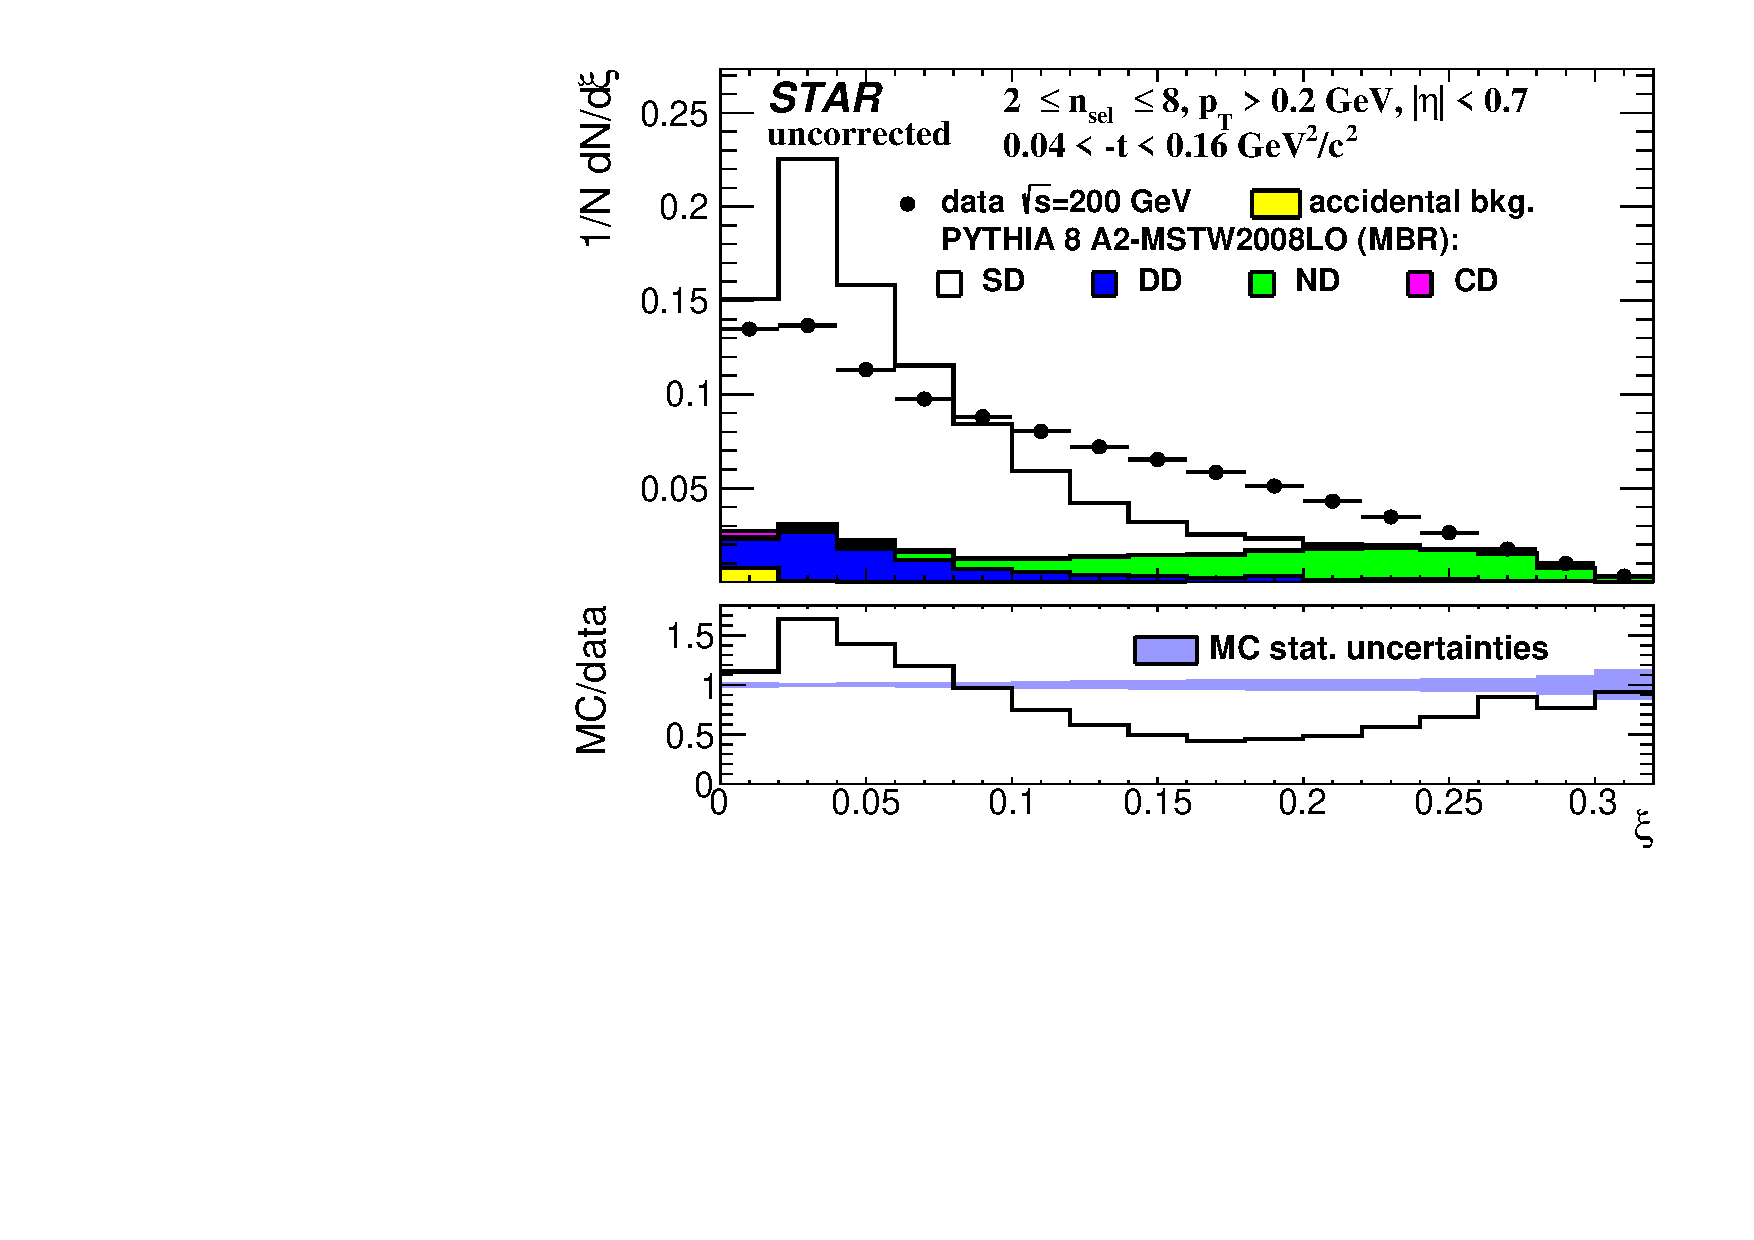
\includegraphics[width=.49\textwidth,page=1]{chapters/chrgSTAR/img/nonSD/SDT_pythia_xi0_RP_starsim_xi.pdf}
	\hfill
	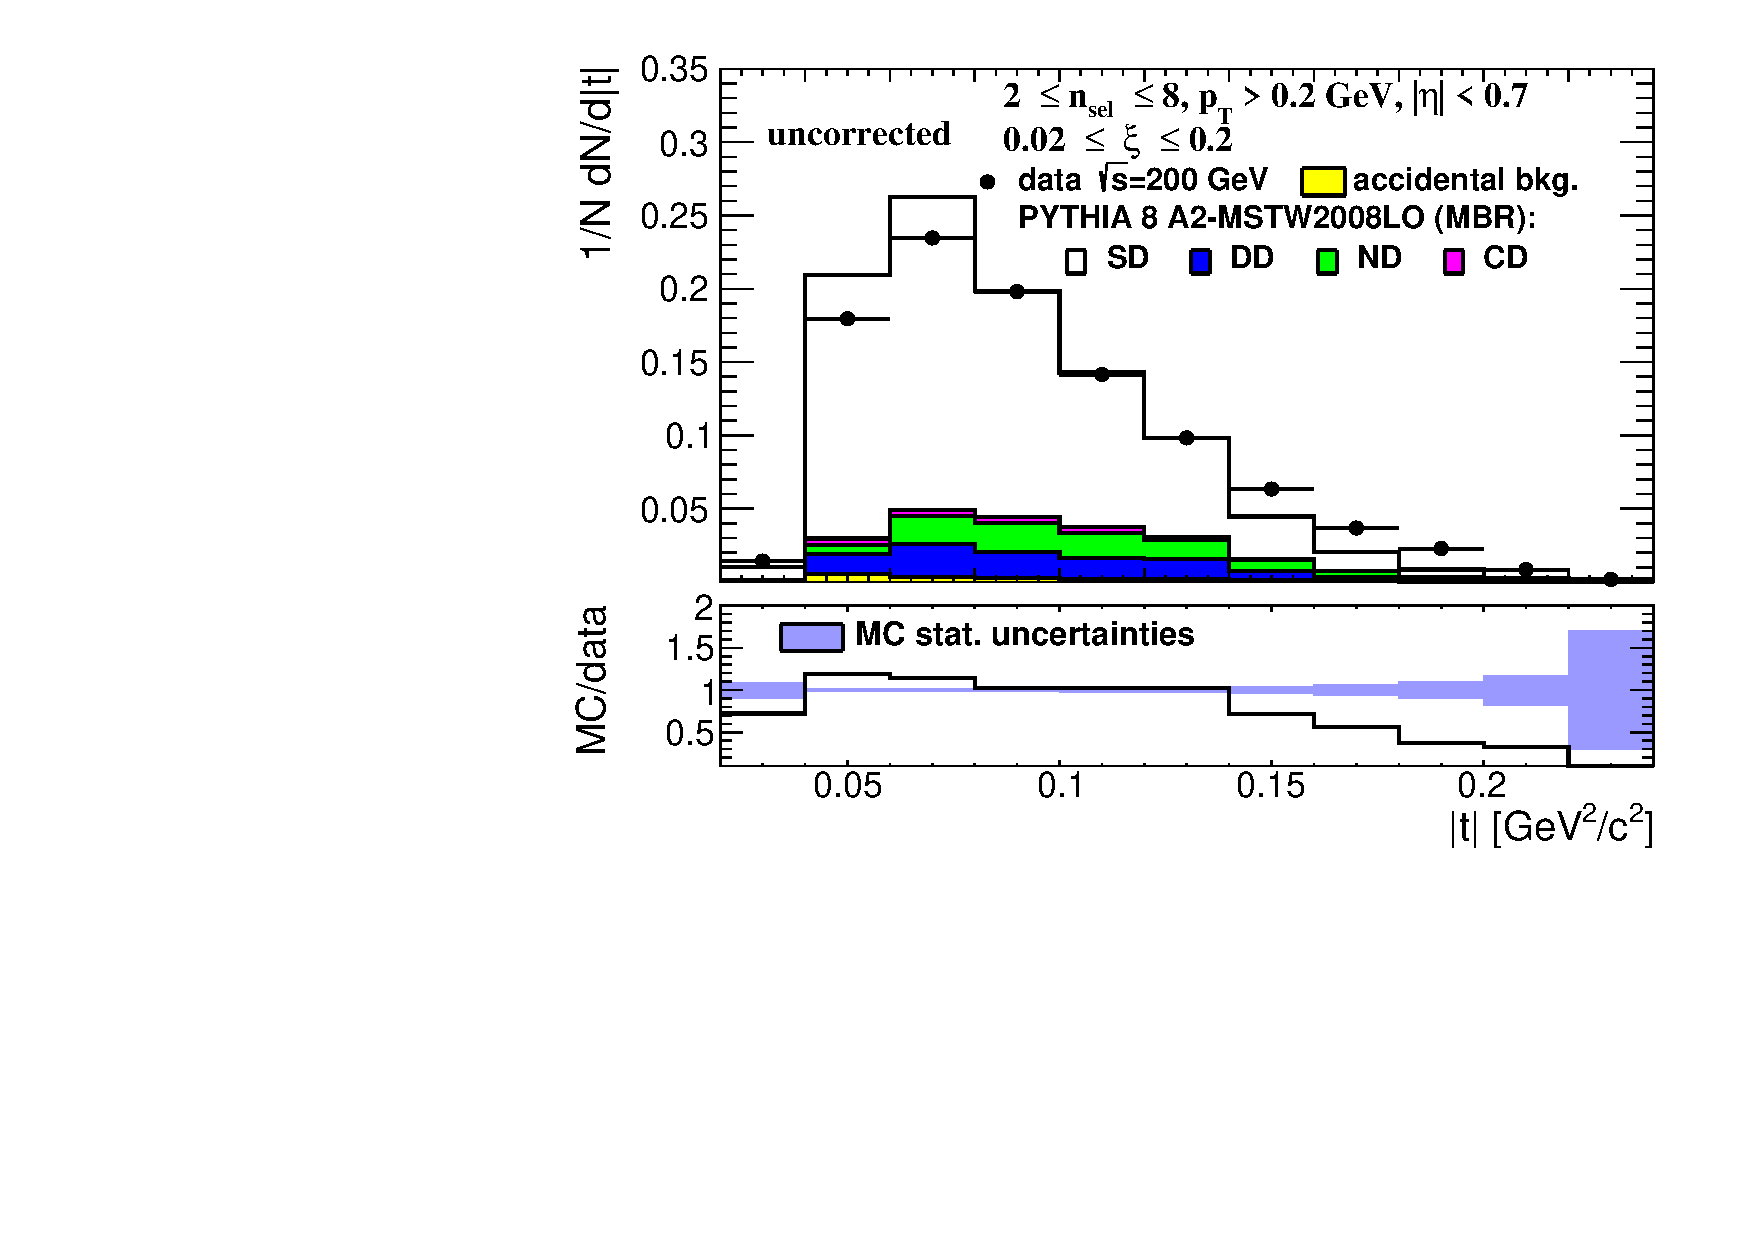
\includegraphics[width=.49\textwidth,page=1]{chapters/chrgSTAR/img/nonSD/SDT_pythia_xi0_RP_starsim_t.pdf}
	\newline
	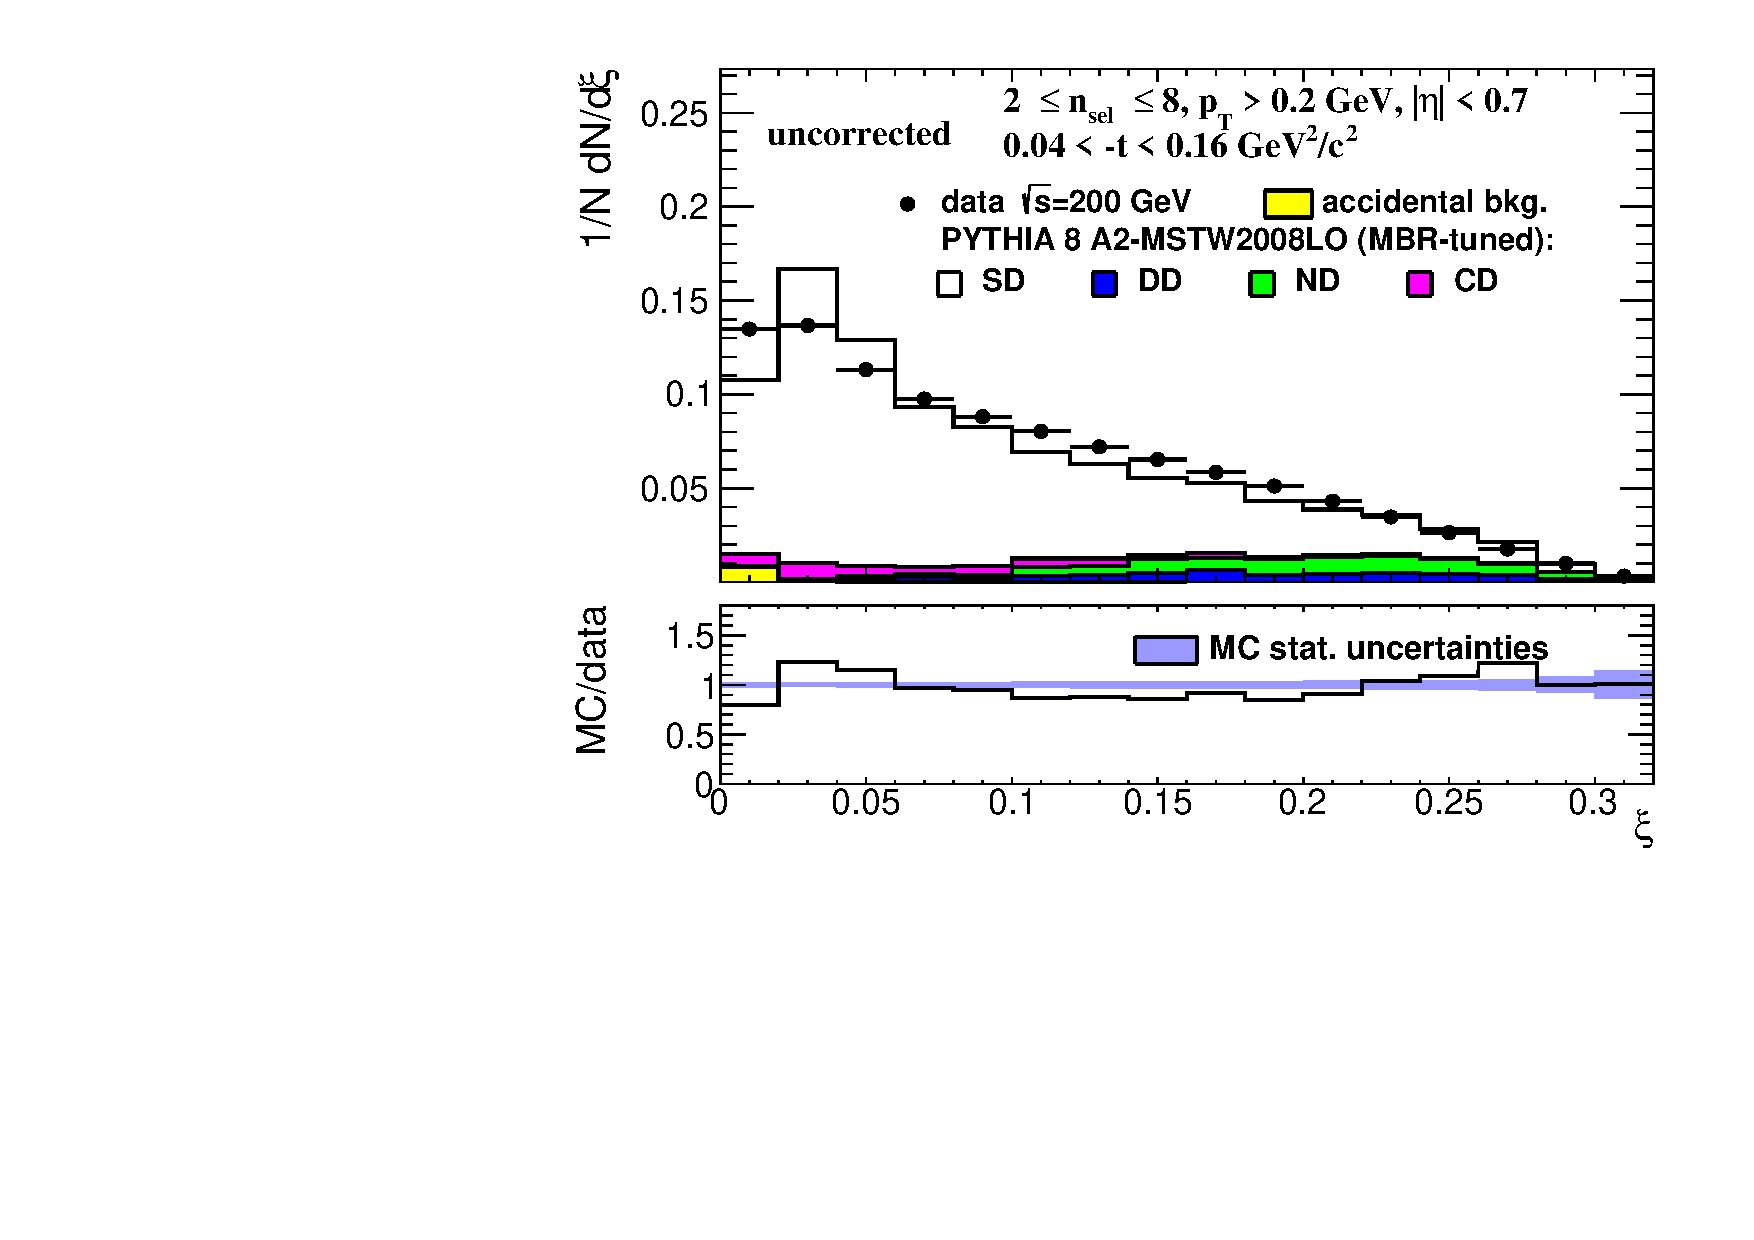
\includegraphics[width=.49\textwidth,page=1]{chapters/chrgSTAR/img/nonSD/SDT_pythia_xi0_option2_RP_starsim_xi.pdf}
	\hfill
	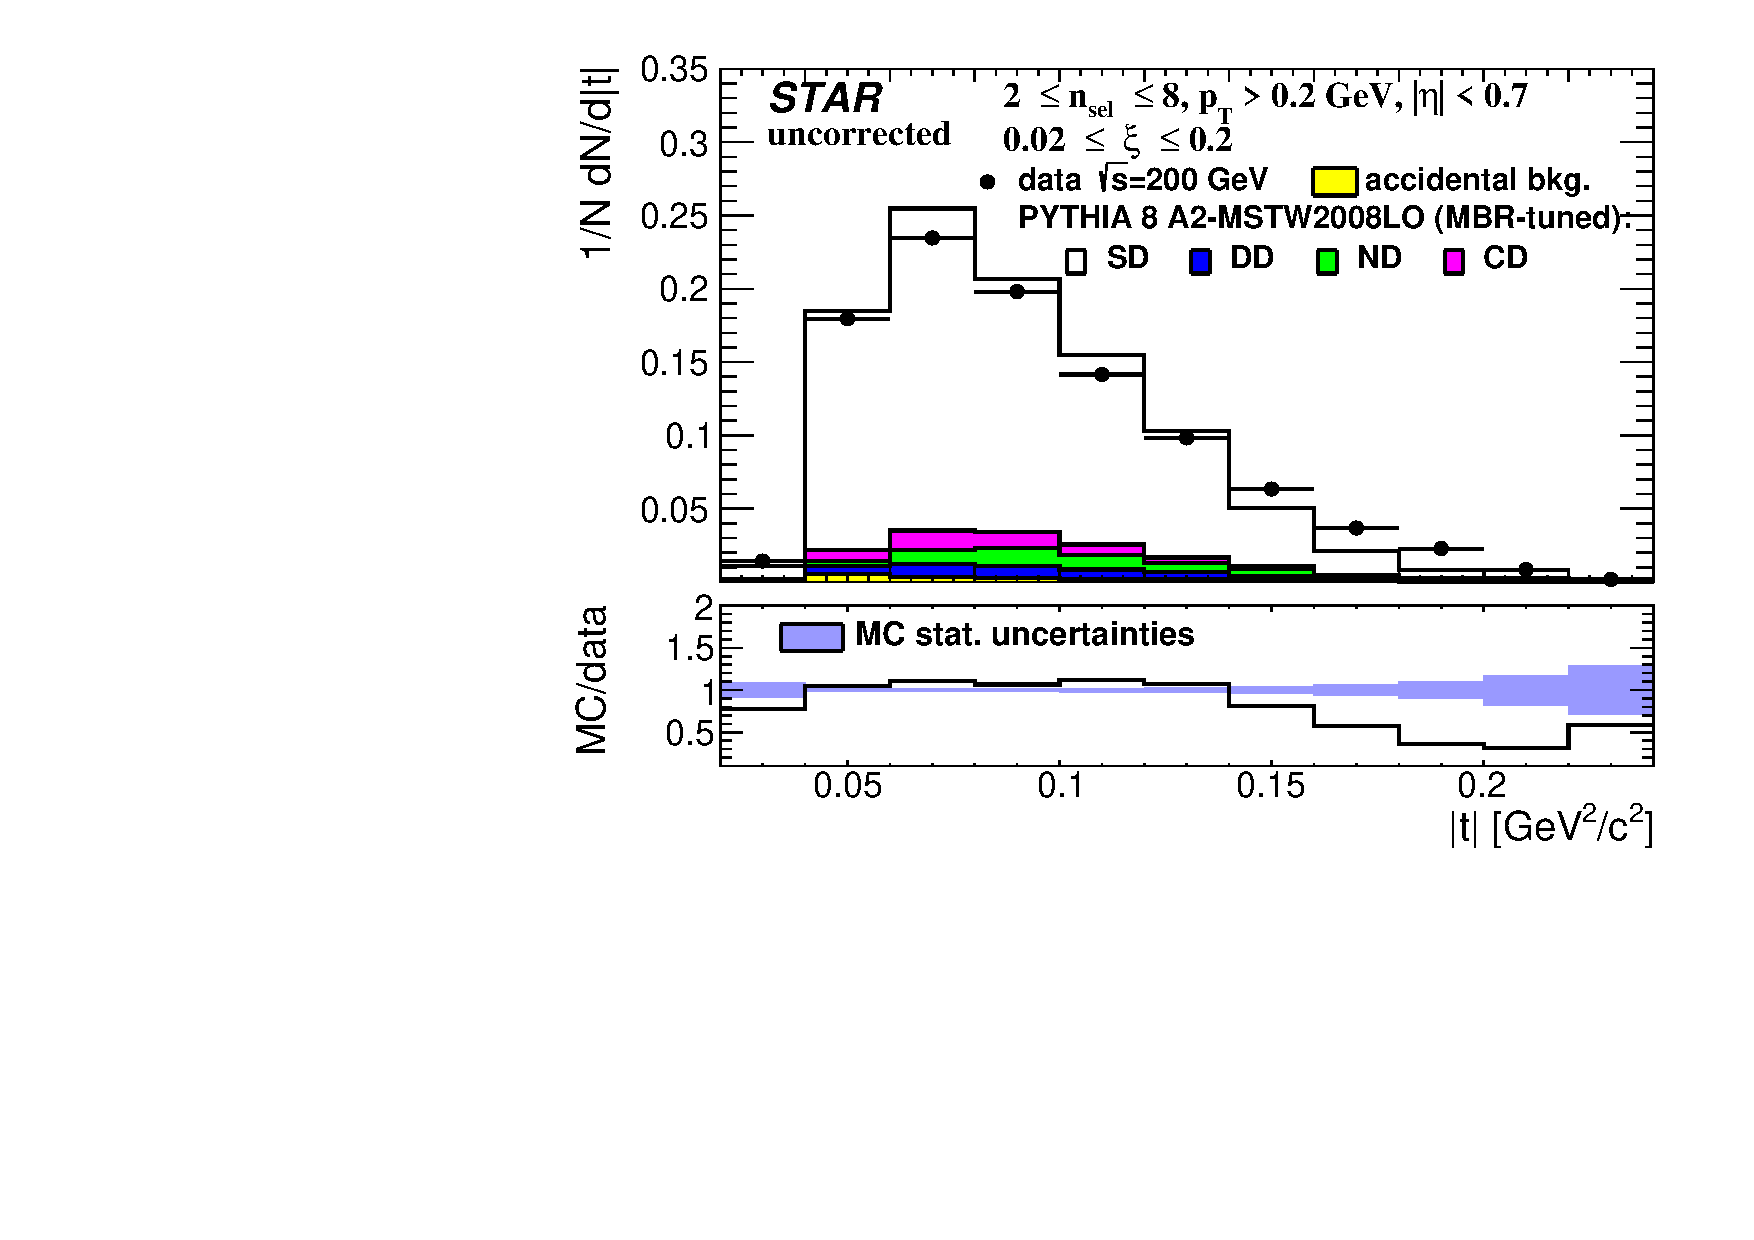
\includegraphics[width=.49\textwidth,page=1]{chapters/chrgSTAR/img/nonSD/SDT_pythia_xi0_option2_RP_starsim_t.pdf}
	\newline
	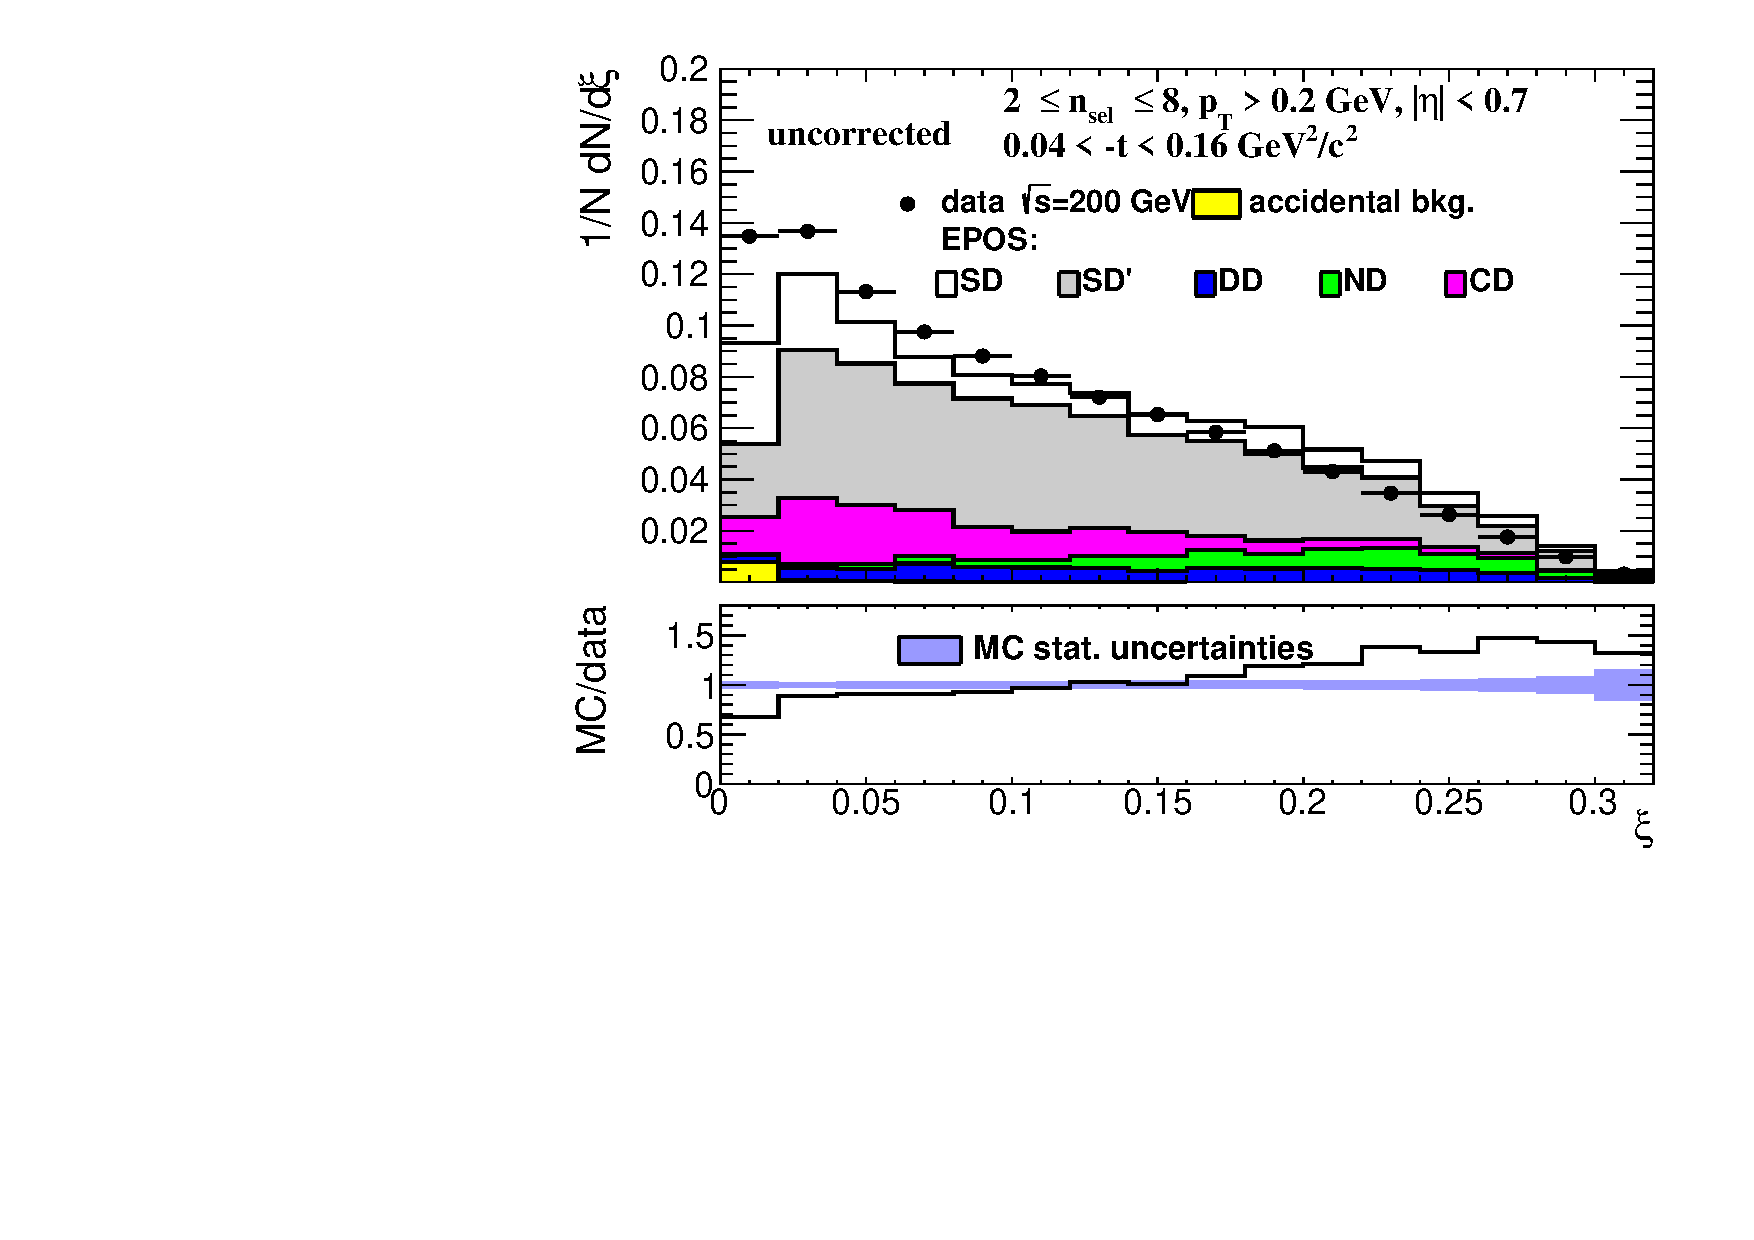
\includegraphics[width=.49\textwidth,page=1]{chapters/chrgSTAR/img/nonSD/SDT_epos_xi0_RP_starsim_xi.pdf}
	\hfill
	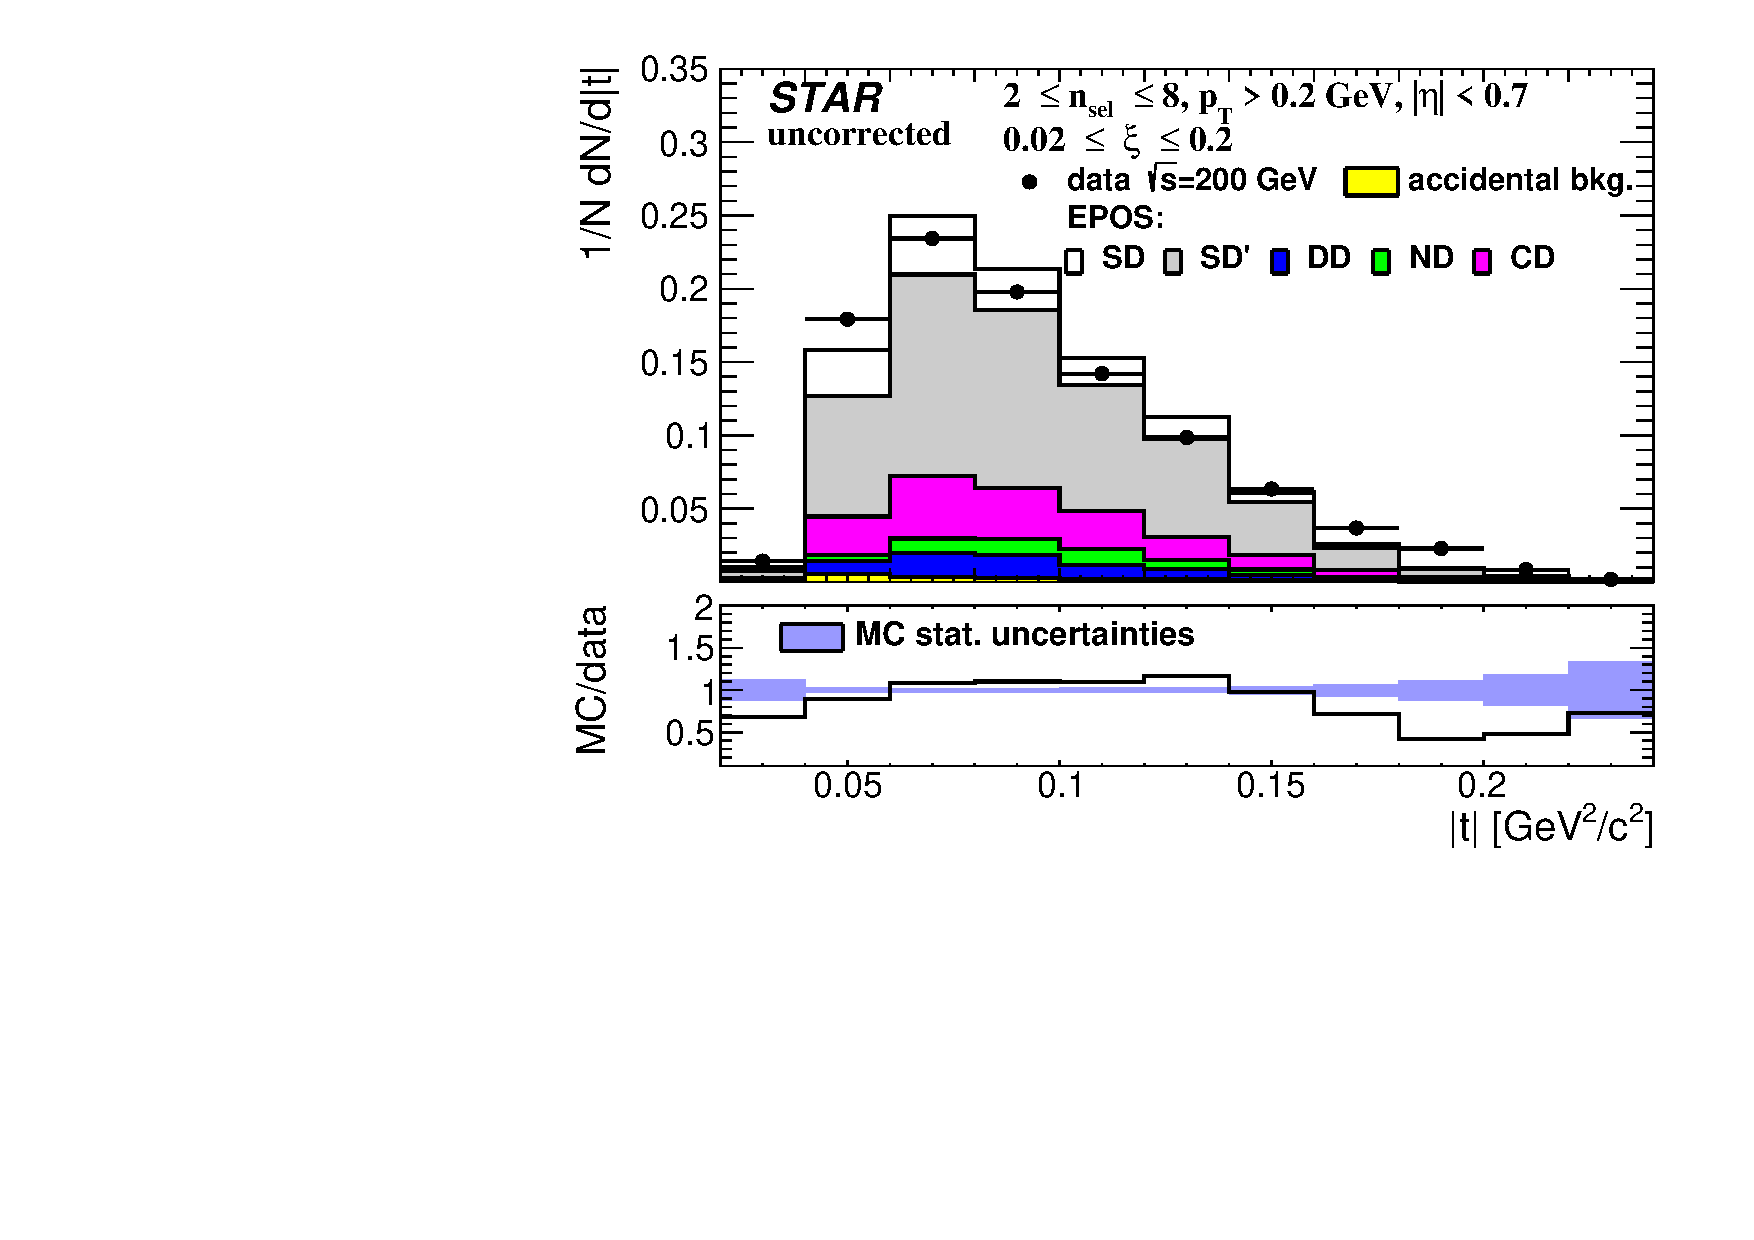
\includegraphics[width=.49\textwidth,page=1]{chapters/chrgSTAR/img/nonSD/SDT_epos_xi0_RP_starsim_t.pdf}
	%
	\caption{Uncorrected distributions of data compared to various MC models: (top) PYTHIA~8 A2 (MBR), (middle) PYTHIA~8 A2 (MBR-tuned) and (bottom) EPOS, as a function of (left column) $\xi$  and (right column) $|t|$.}
	\label{fig:nonSDxit}
	\vspace{-1.5cm}
\end{figure}
%\newpage

\begin{figure}[h!]
	\centering
	\begin{subfigure}{.49\textwidth}
		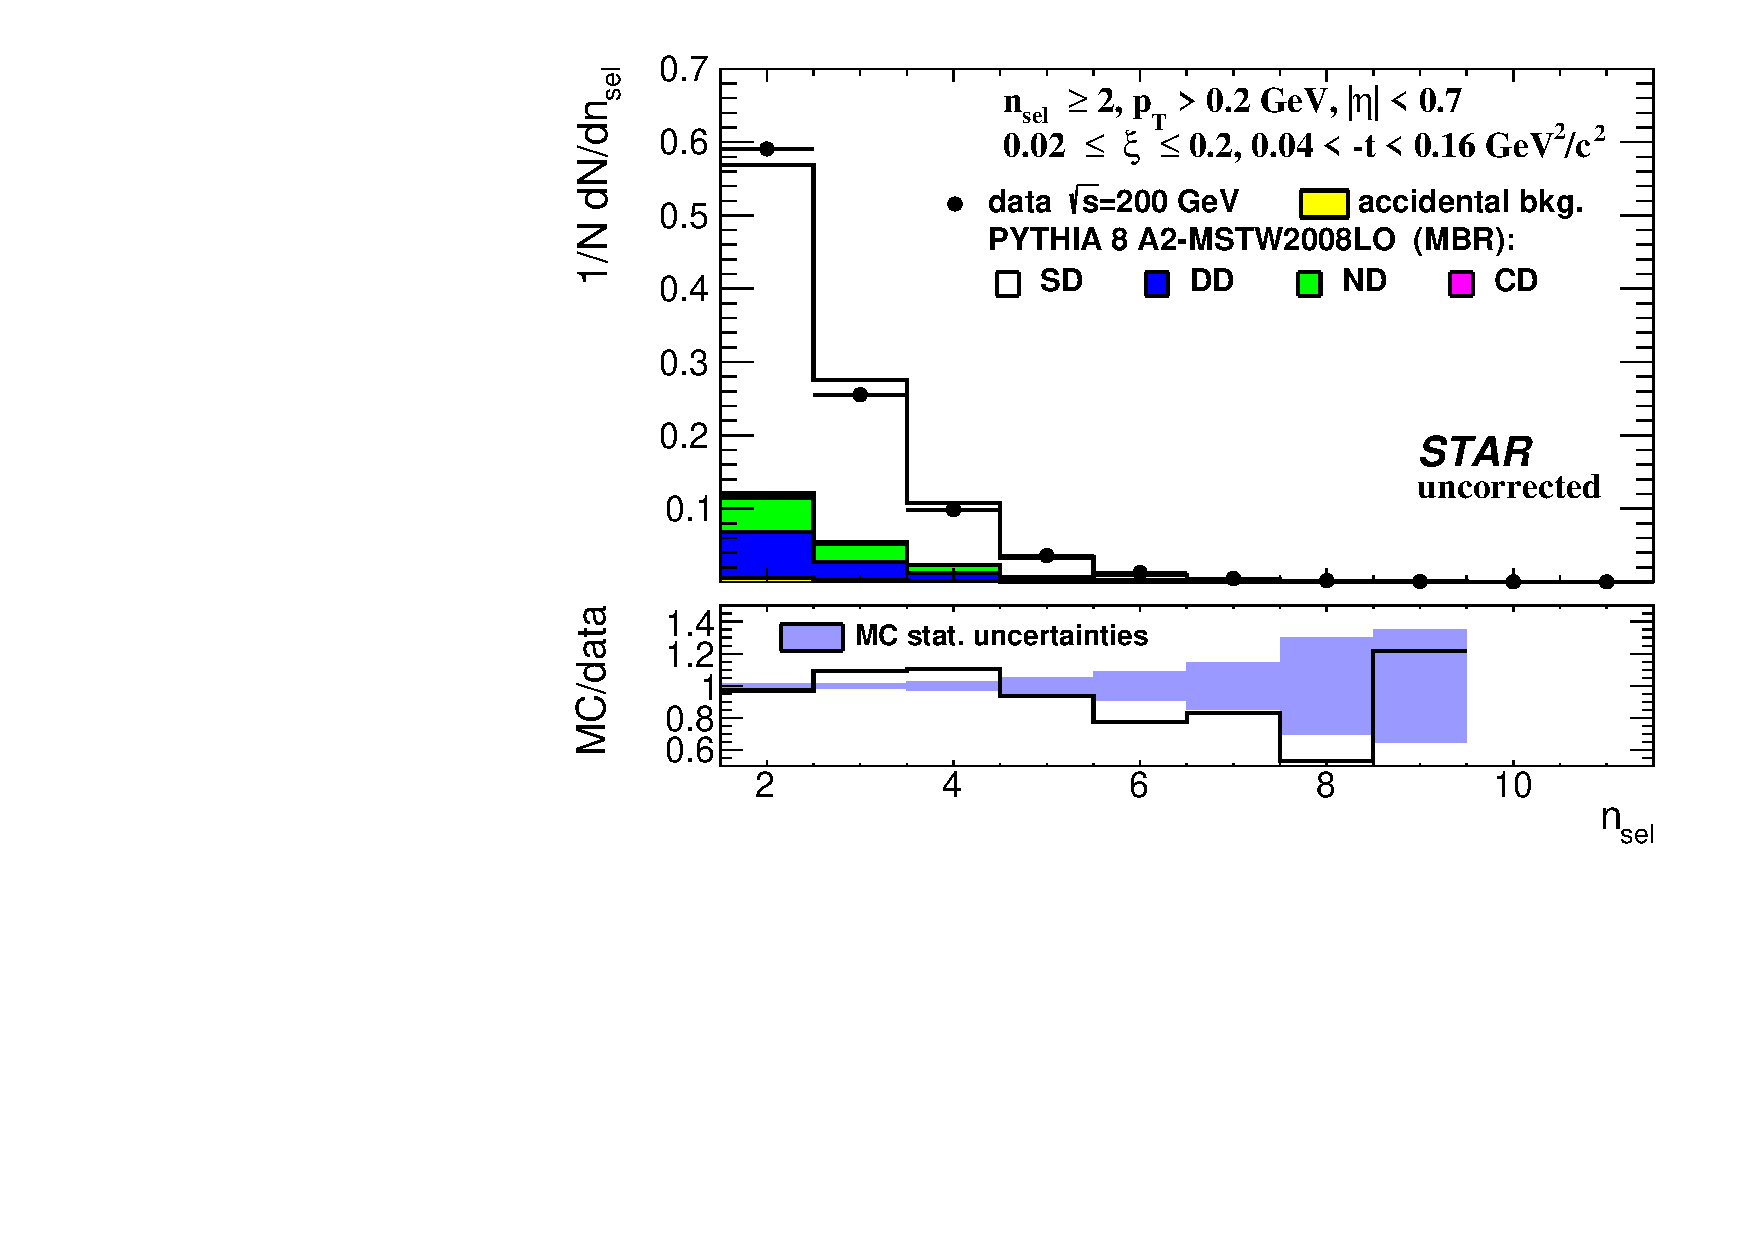
\includegraphics[width=\linewidth, page=1]{chapters/chrgSTAR/img/nonSD/chrg/SDT_pythia_xi0_RP_starsim_nsel.pdf}
	\end{subfigure}
	\begin{subfigure}{.49\textwidth}
		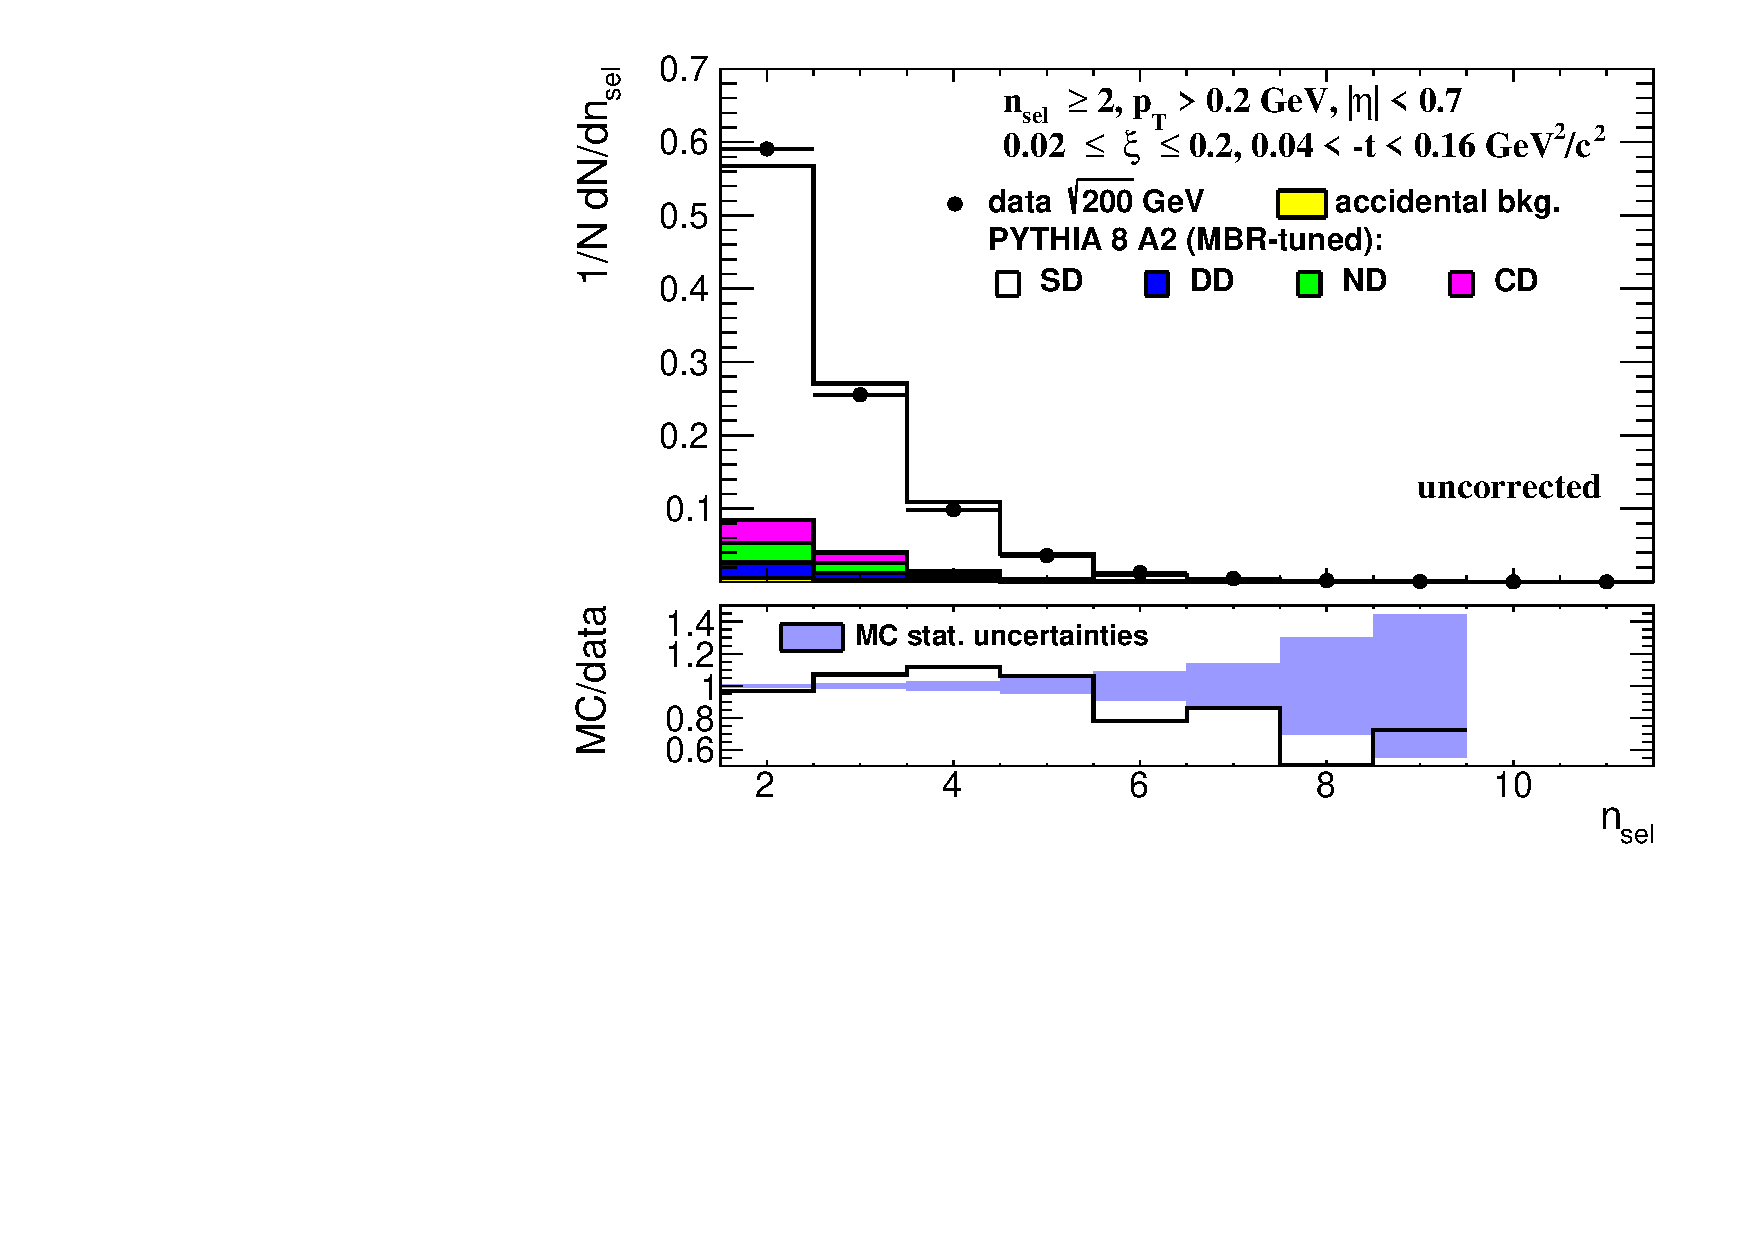
\includegraphics[width=\linewidth, page=1]{chapters/chrgSTAR/img/nonSD/chrg/SDT_pythia_xi0_option2_RP_starsim_nsel.pdf}
	\end{subfigure}
	\begin{subfigure}{.49\textwidth}
		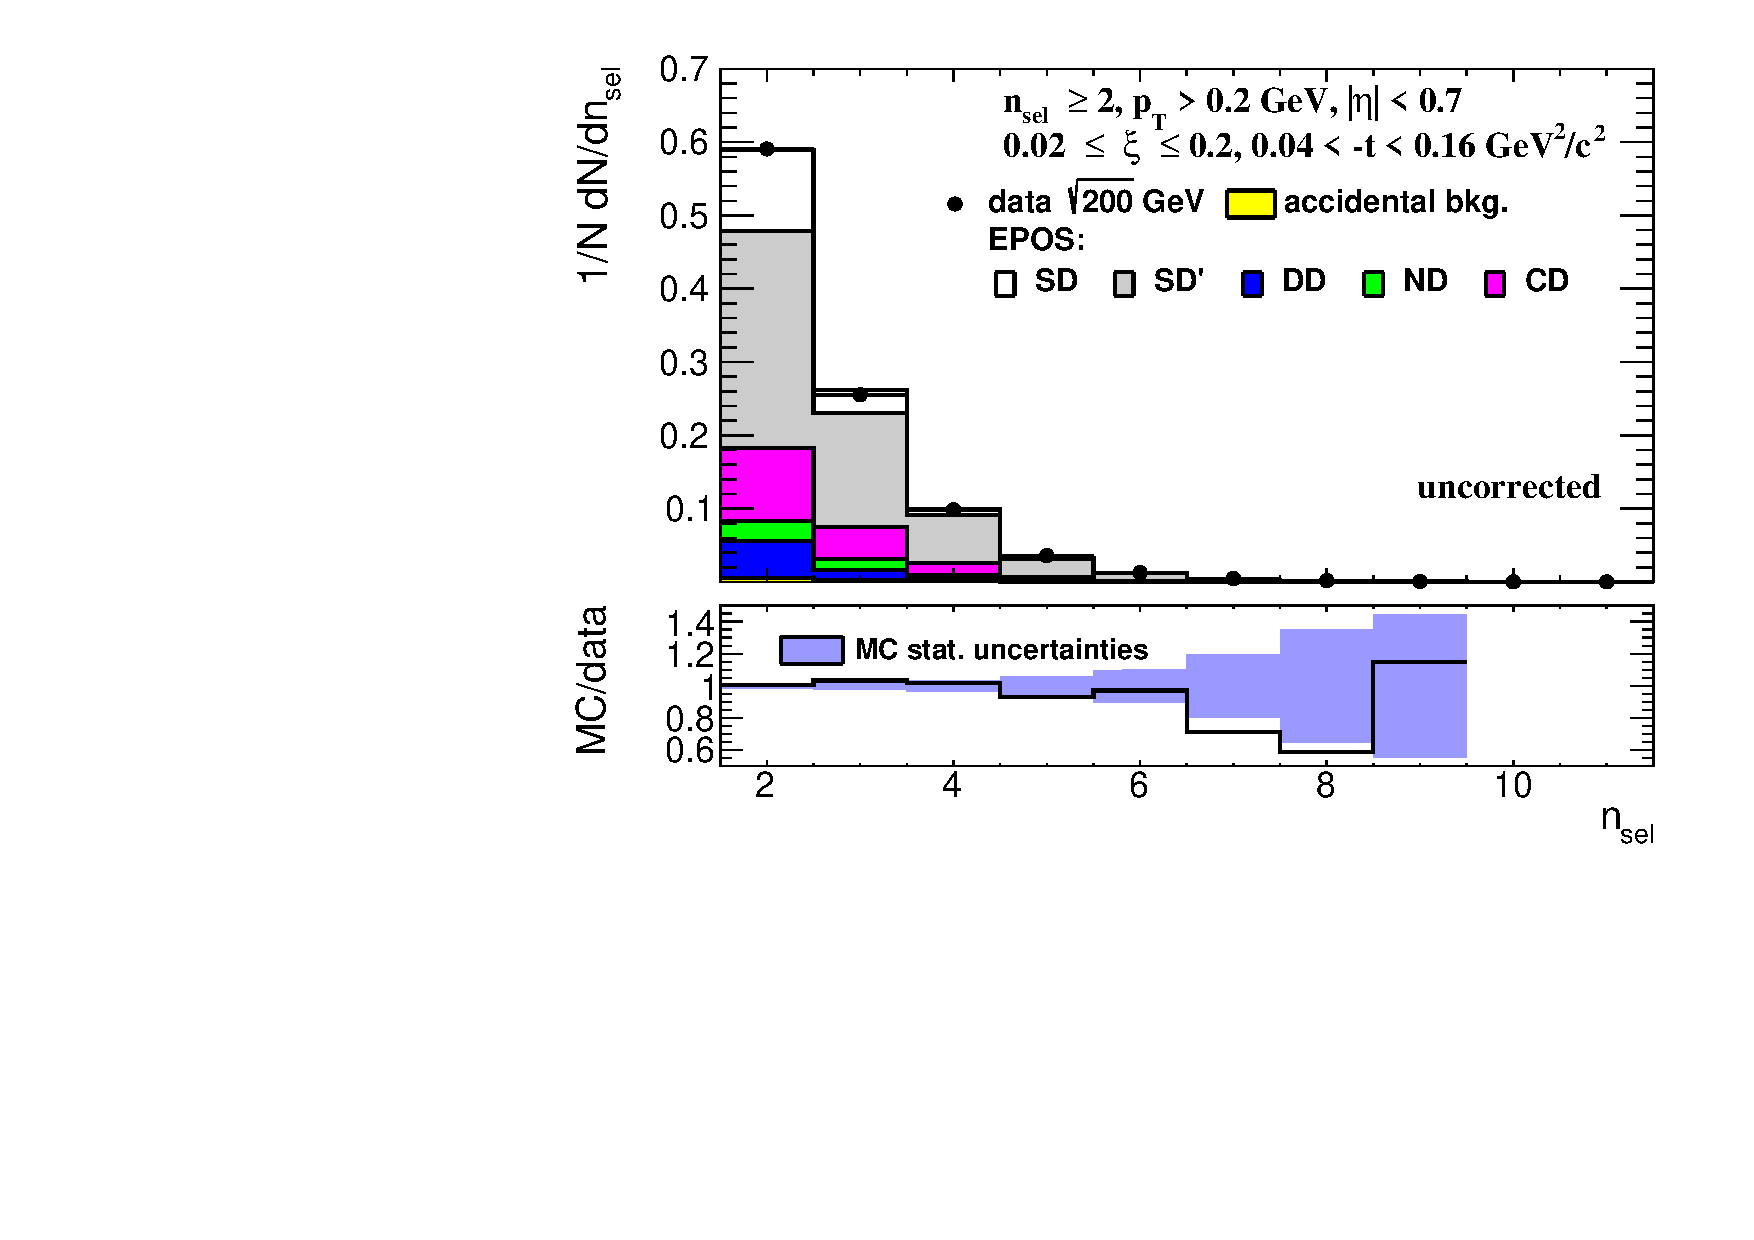
\includegraphics[width=\linewidth, page=1]{chapters/chrgSTAR/img/nonSD/chrg/SDT_epos_xi0_RP_starsim_nsel.pdf}
	\end{subfigure}
	\begin{minipage}{.49\textwidth}
		\caption{Uncorrected distributions of data compared to various MC models: (top left) PYTHIA~8 A2 (MBR), (top right) PYTHIA~8 A2 (MBR-tuned) and (bottom) EPOS, as a function of $n_{\mathrm{sel}}$.}
		\label{fig:nonSDnsel}
	\end{minipage}
	
\end{figure}
\begin{figure}[h!]
%	\vspace{-0.5cm}
	\centering
	\begin{subfigure}{.49\textwidth}
		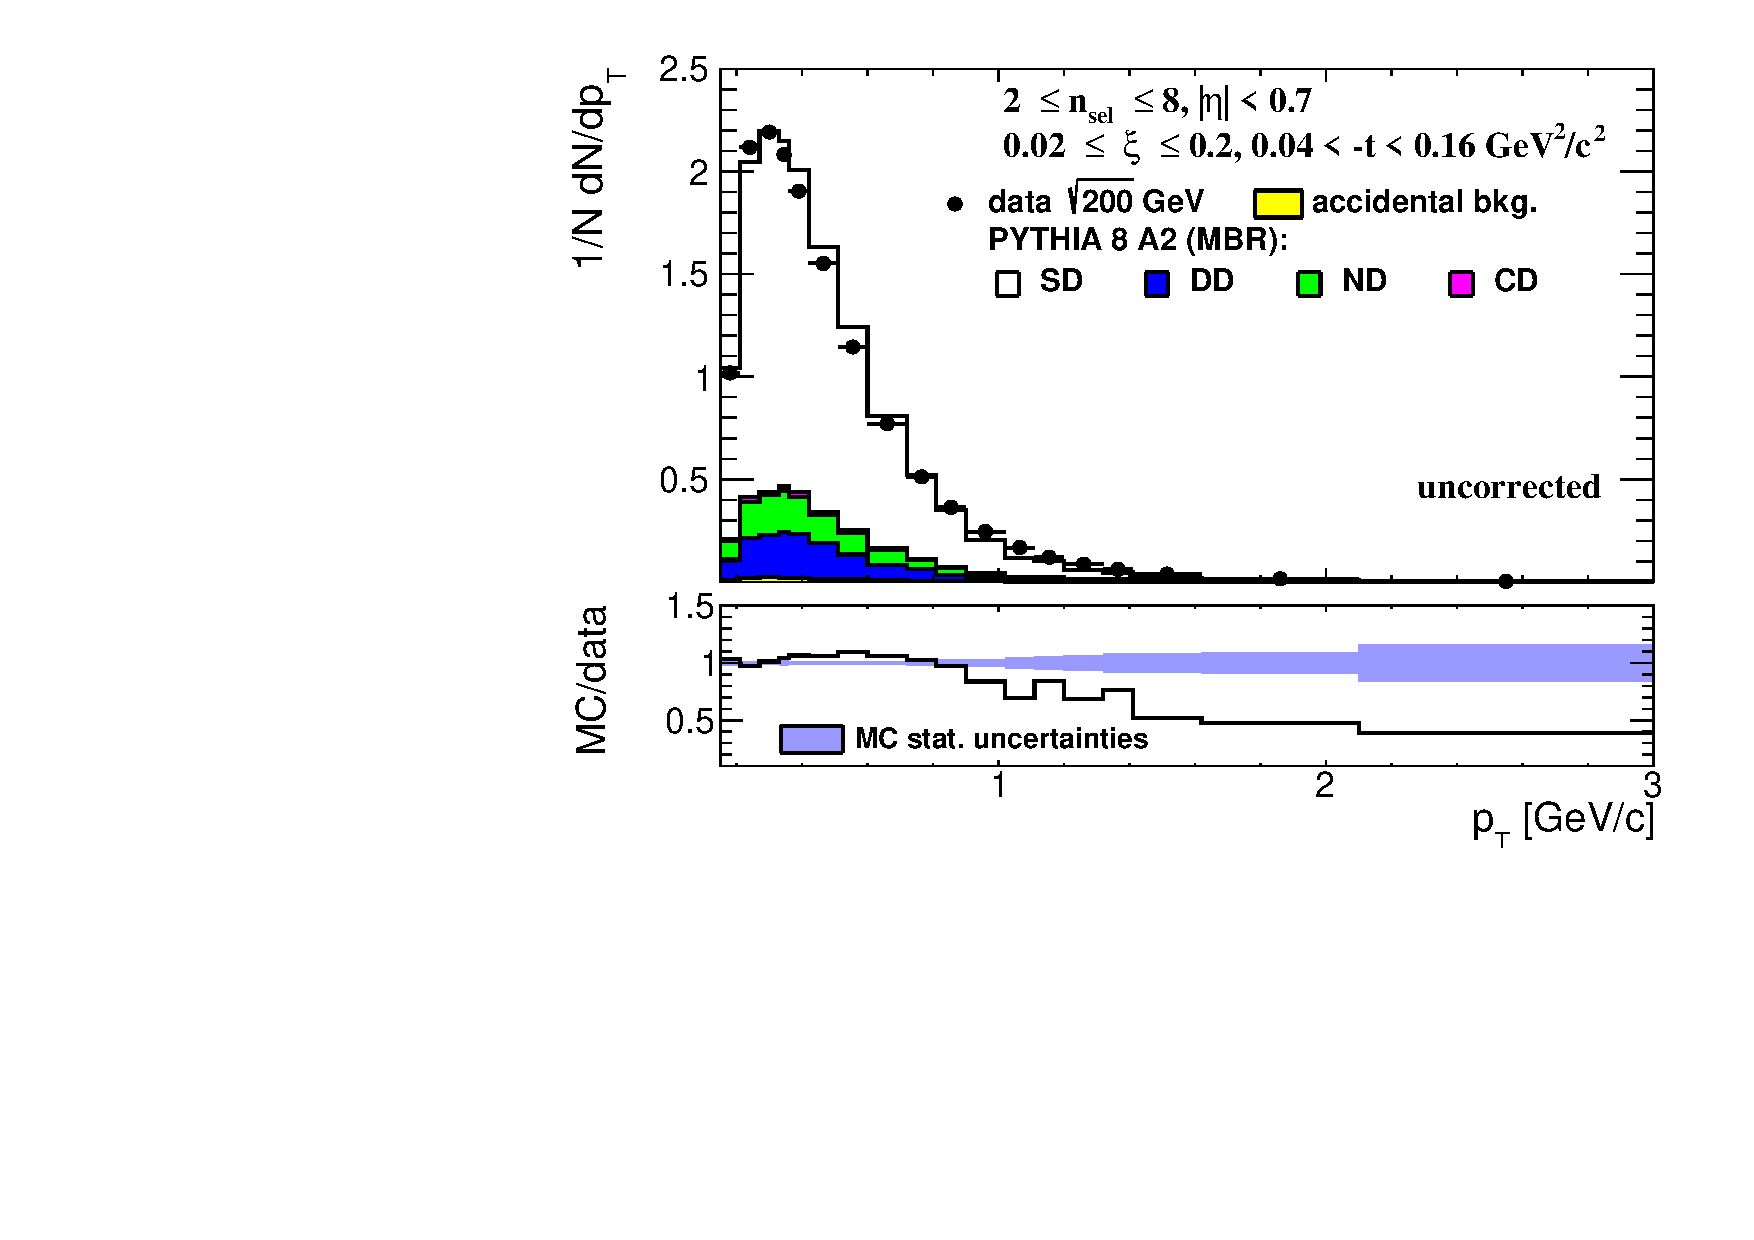
\includegraphics[width=\linewidth, page=1]{chapters/chrgSTAR/img/nonSD/chrg/SDT_pythia_xi0_RP_starsim_pt.pdf}
	\end{subfigure}
	\begin{subfigure}{.49\textwidth}
		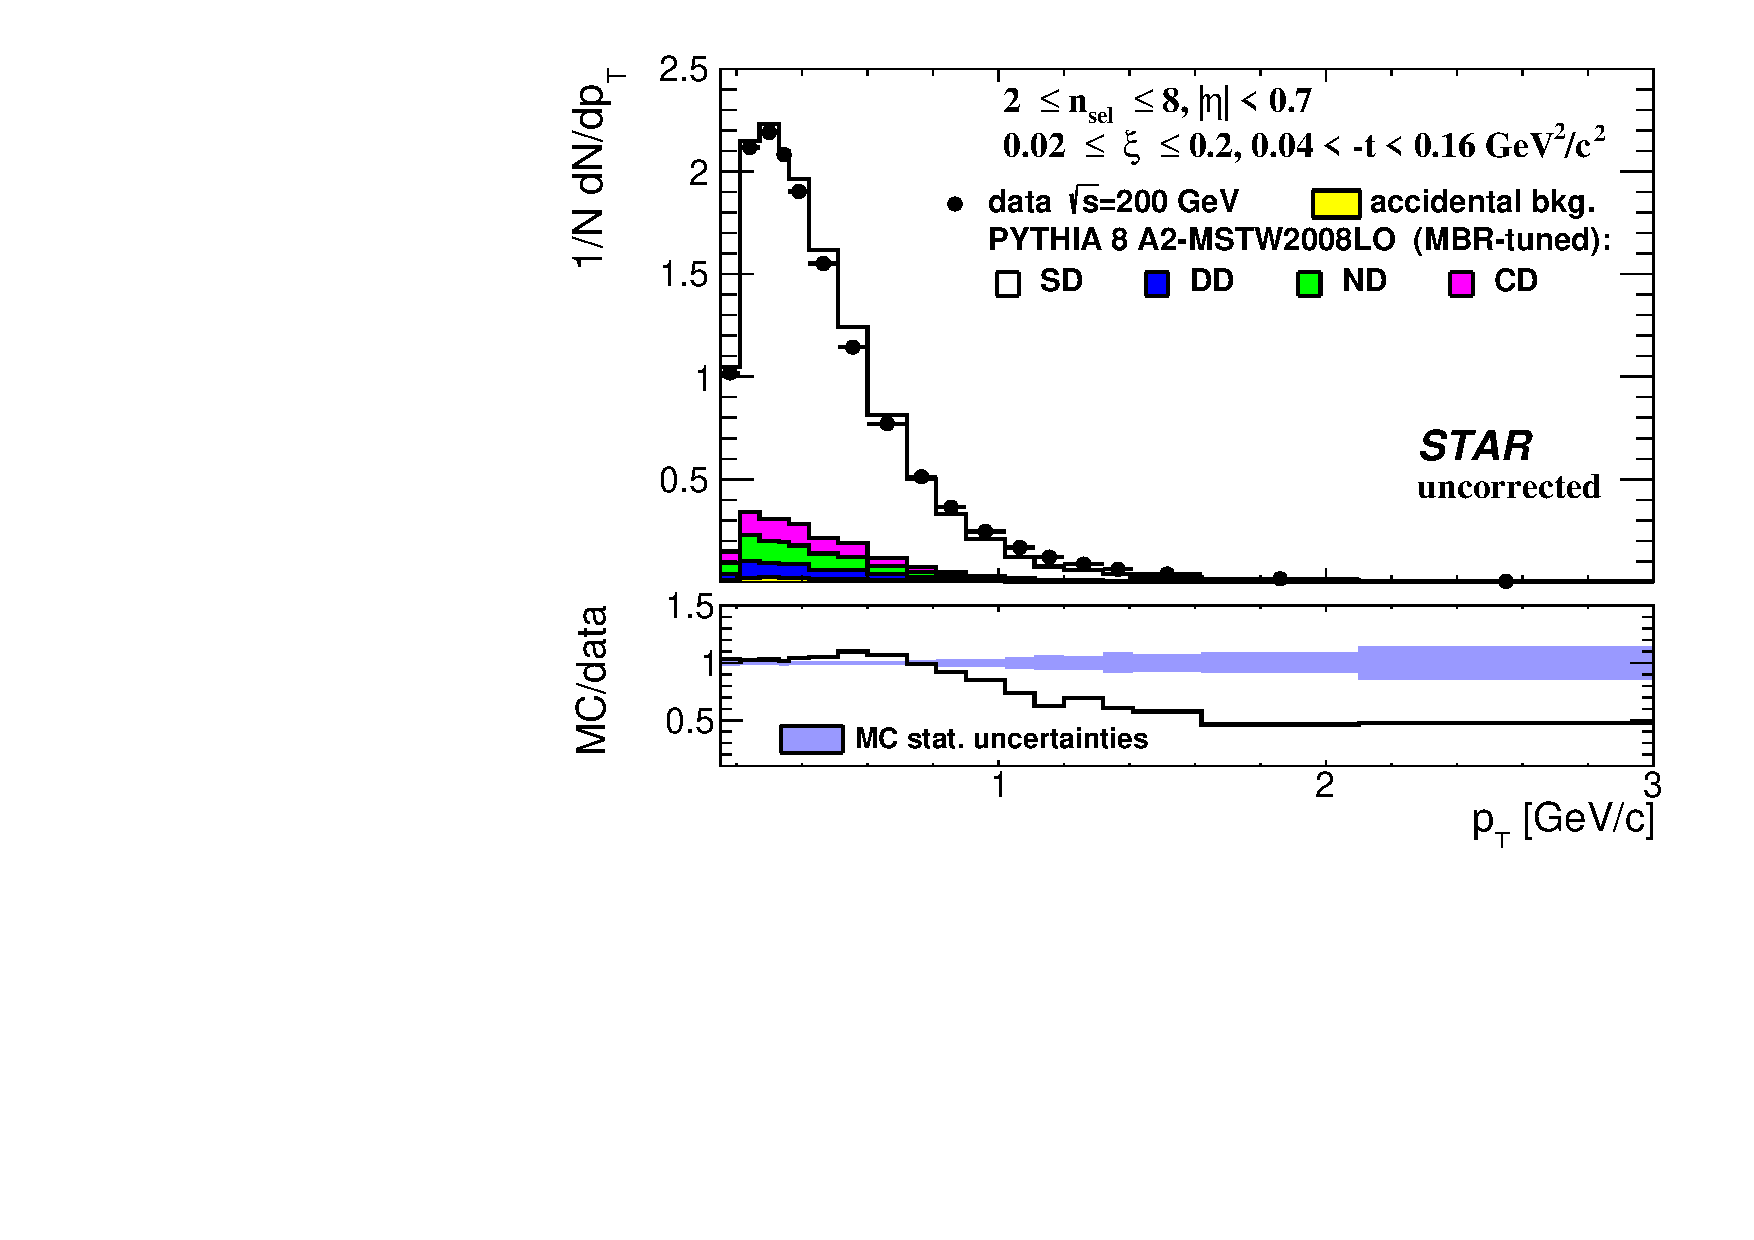
\includegraphics[width=\linewidth, page=1]{chapters/chrgSTAR/img/nonSD/chrg/SDT_pythia_xi0_option2_RP_starsim_pt.pdf}
	\end{subfigure}
	\begin{subfigure}{.49\textwidth}
		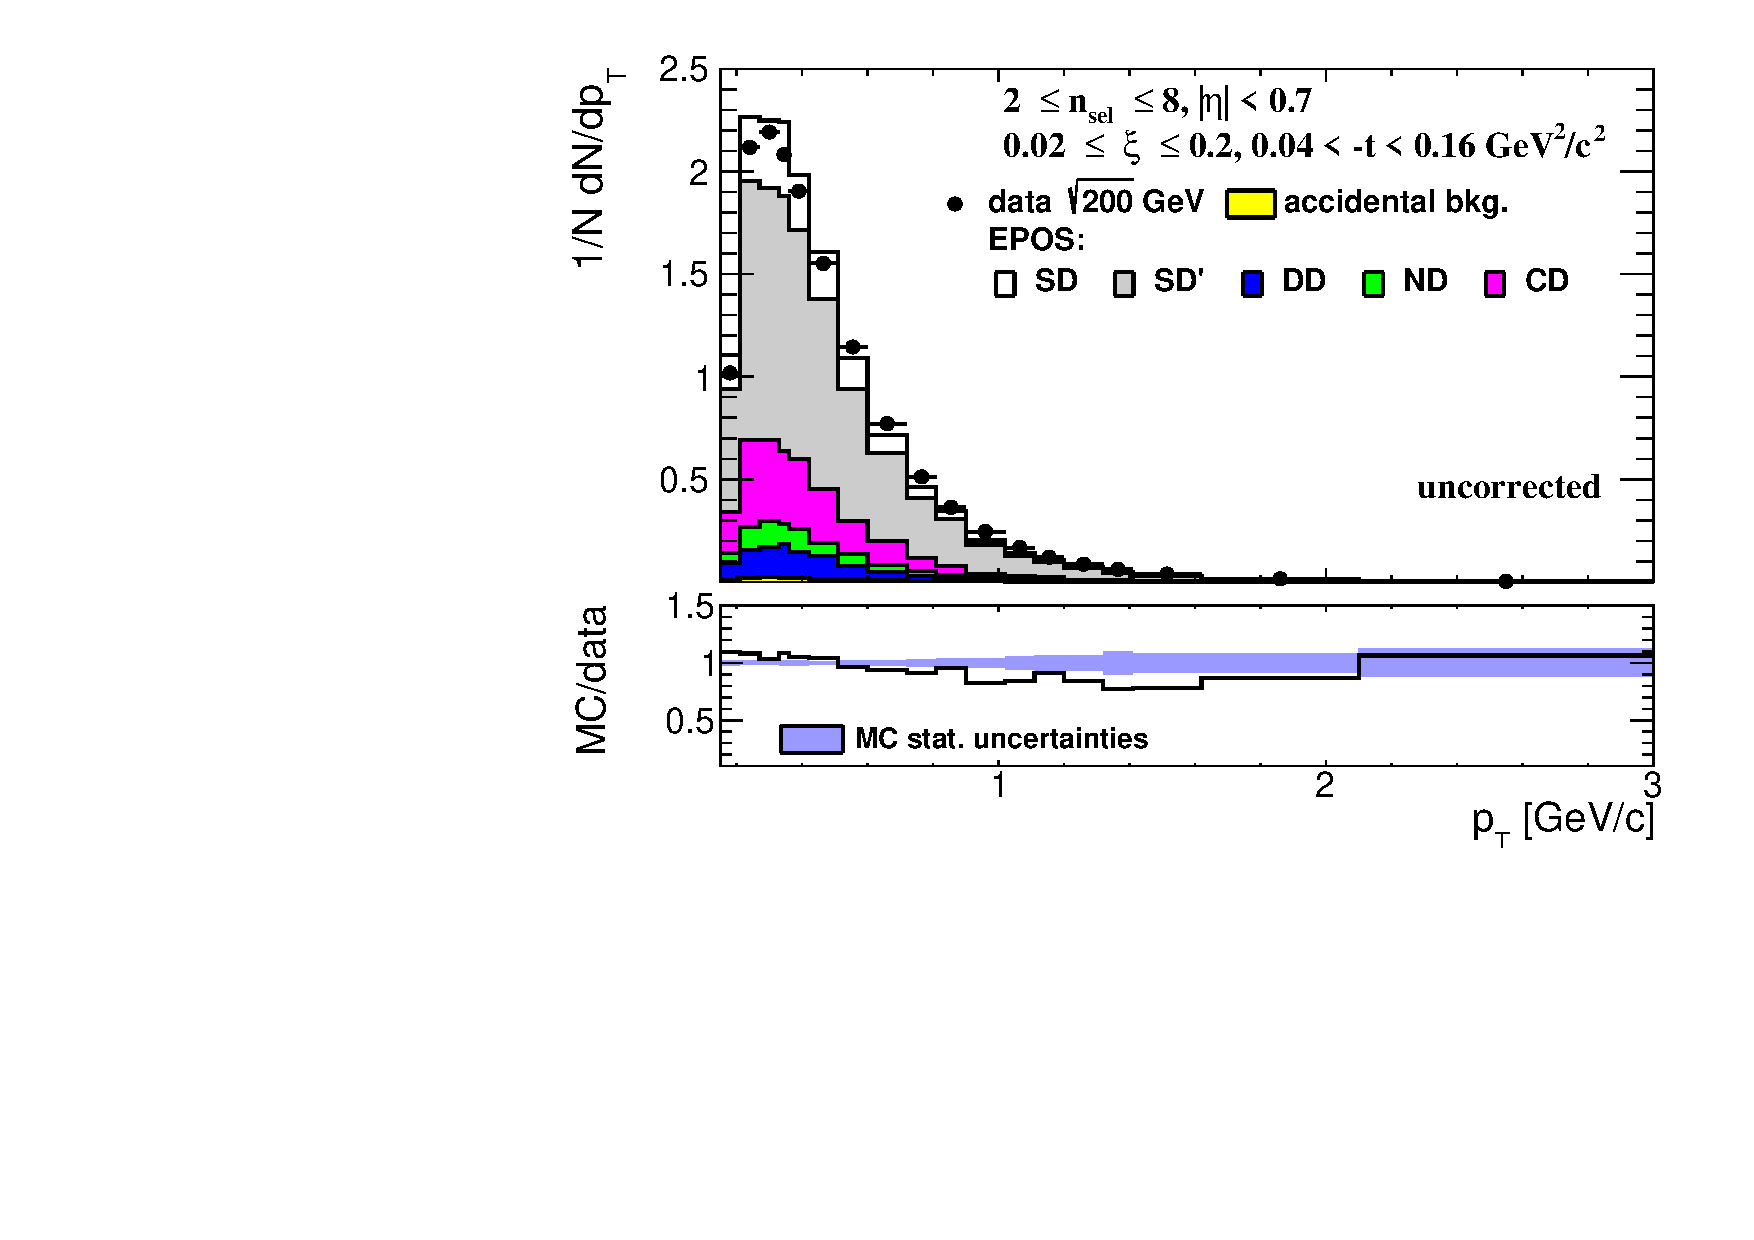
\includegraphics[width=\linewidth, page=1]{chapters/chrgSTAR/img/nonSD/chrg/SDT_epos_xi0_RP_starsim_pt.pdf}
	\end{subfigure}
	\begin{minipage}{.49\textwidth}
		\caption{Uncorrected distributions of data compared to various MC models: (top left) PYTHIA~8 A2 (MBR), (top right) PYTHIA~8 A2 (MBR-tuned) and (bottom) EPOS, as a function of $p_{\mathrm{T}}$.}
		\label{fig:nonSDpt}
	\end{minipage}
	
\end{figure}
%\newpage
\begin{figure}[h!]
%	\vspace{-0.5cm}
	\centering
	\begin{subfigure}{.49\textwidth}
		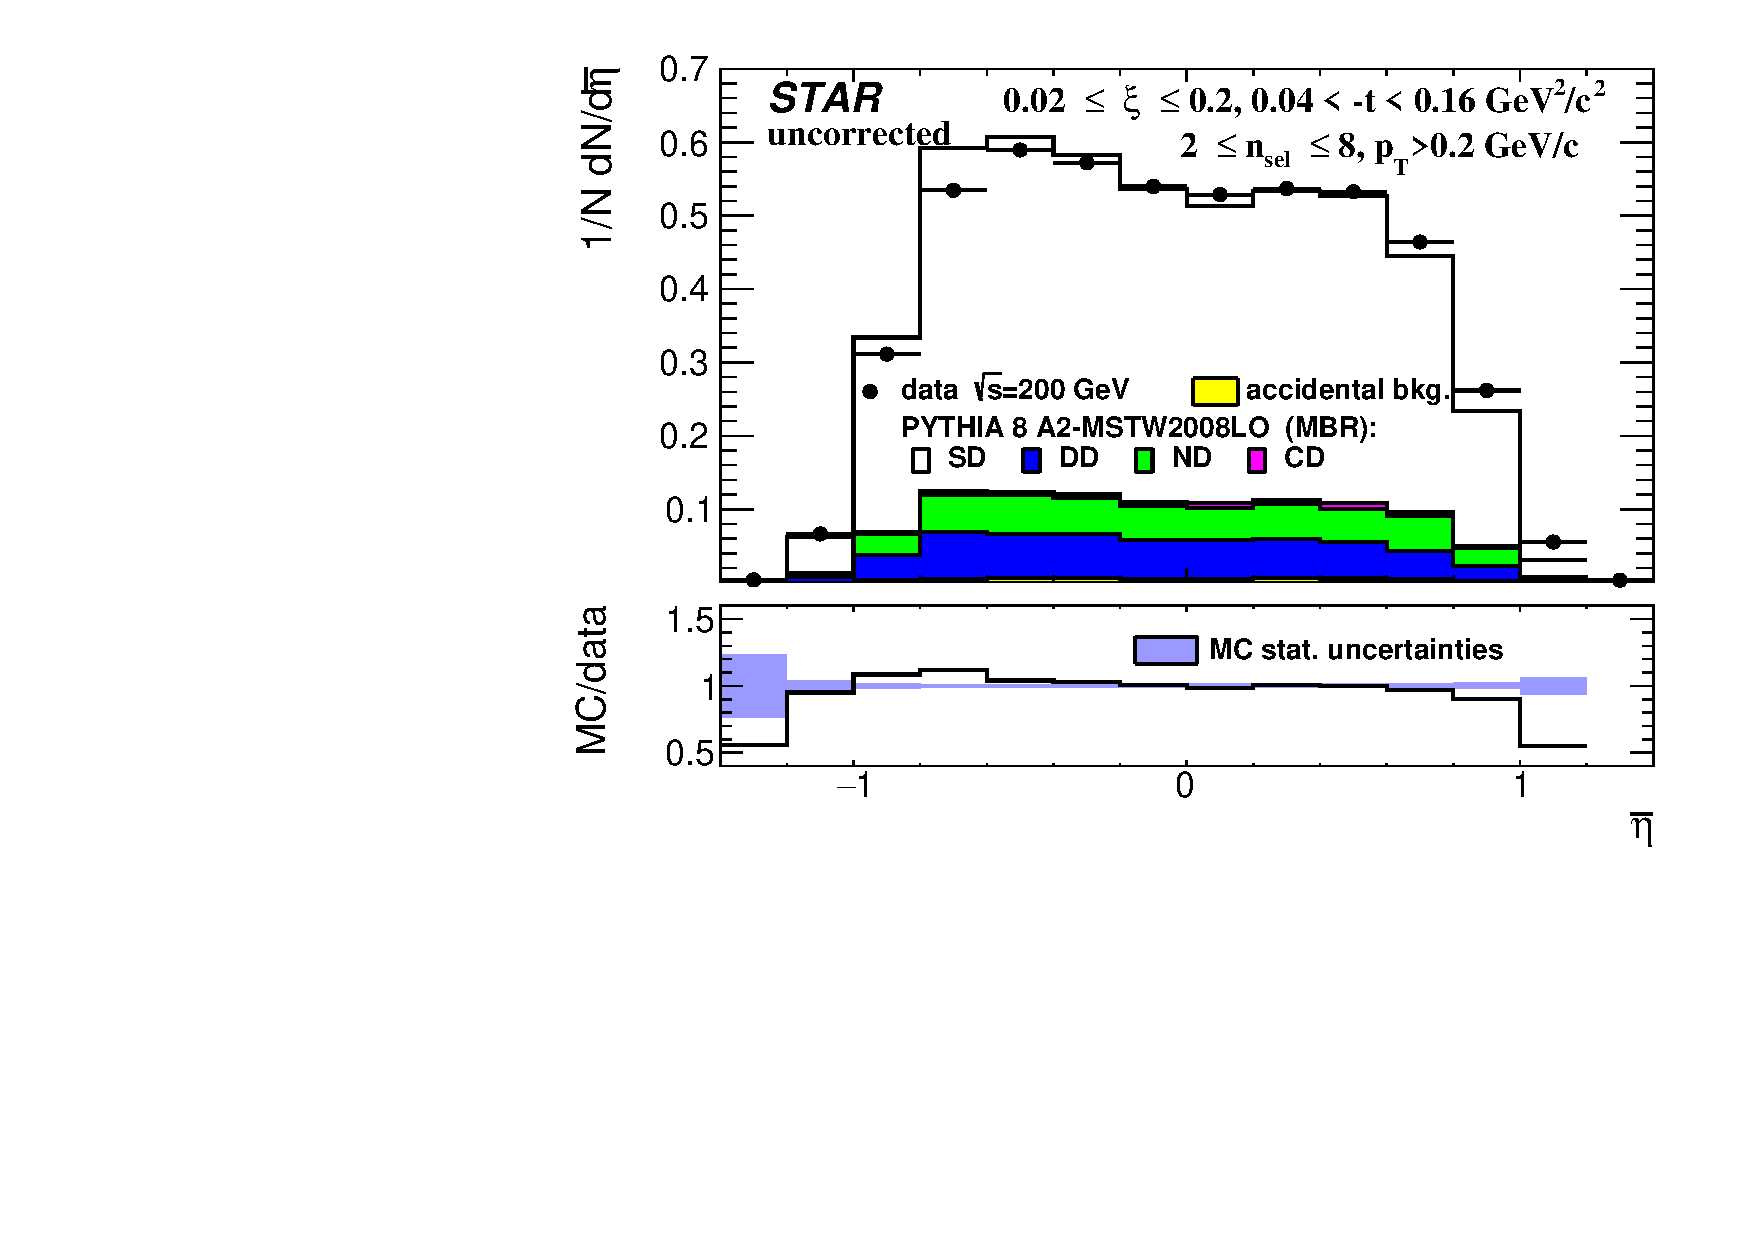
\includegraphics[width=\linewidth, page=1]{chapters/chrgSTAR/img/nonSD/chrg/SDT_pythia_xi0_RP_starsim_eta.pdf}
	\end{subfigure}
	\begin{subfigure}{.49\textwidth}
		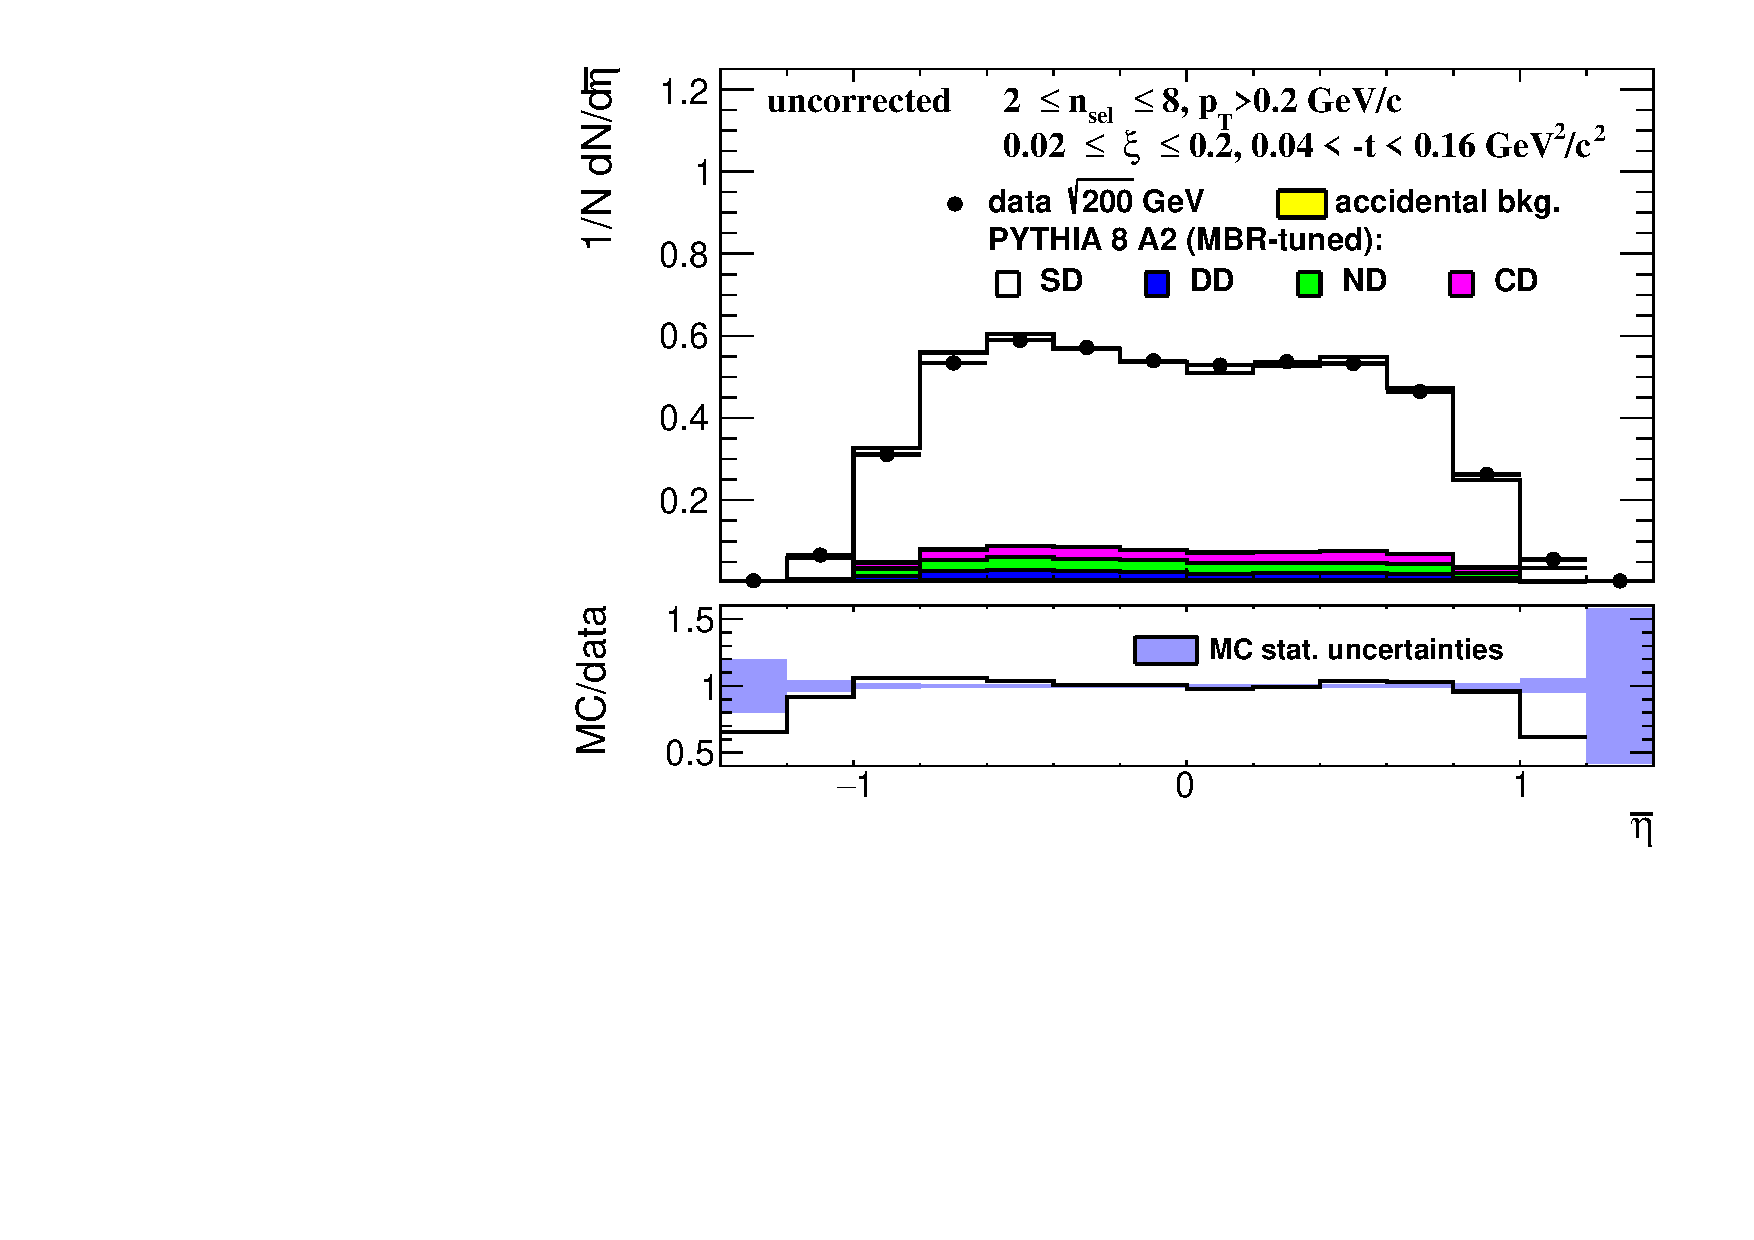
\includegraphics[width=\linewidth, page=1]{chapters/chrgSTAR/img/nonSD/chrg/SDT_pythia_xi0_option2_RP_starsim_eta.pdf}
	\end{subfigure}
	\begin{subfigure}{.49\textwidth}
		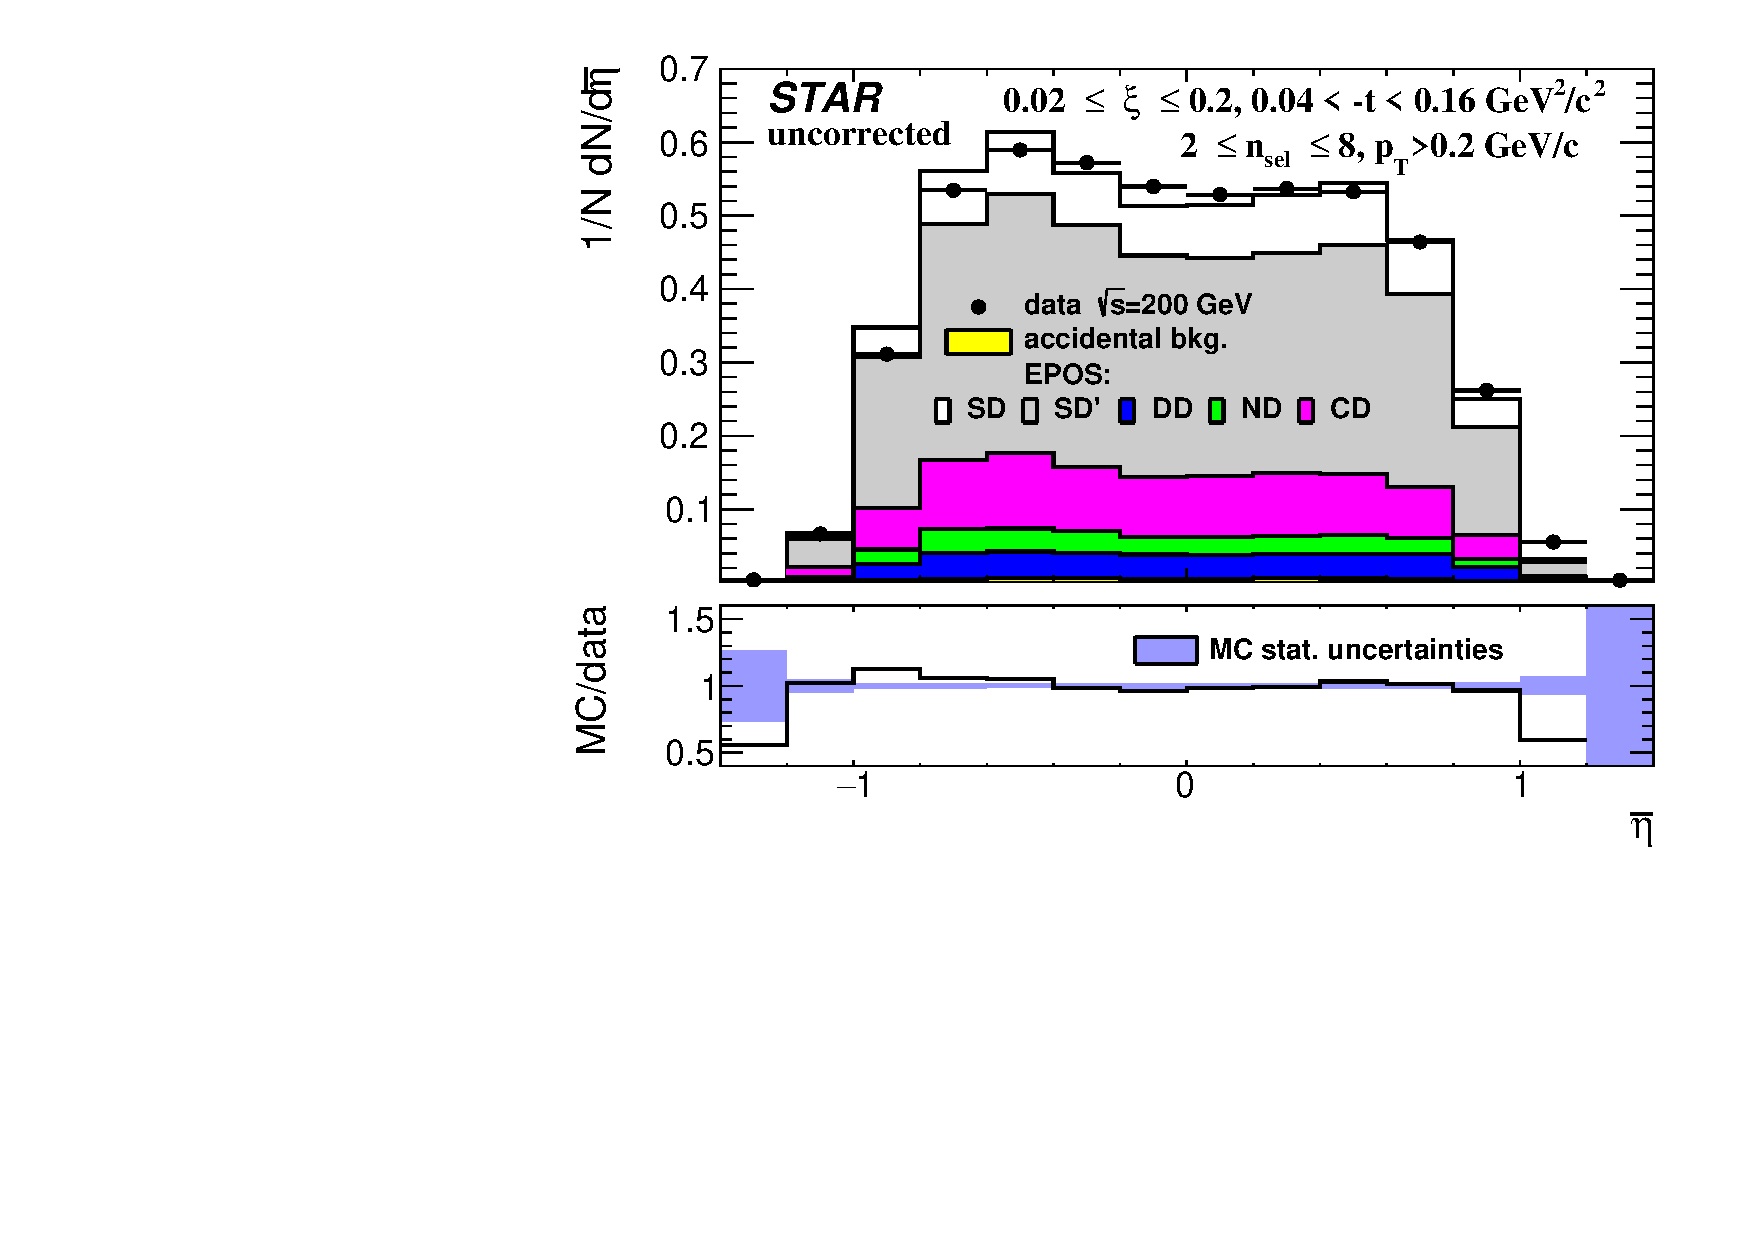
\includegraphics[width=\linewidth, page=1]{chapters/chrgSTAR/img/nonSD/chrg/SDT_epos_xi0_RP_starsim_eta.pdf}
	\end{subfigure}
	\begin{minipage}{.49\textwidth}
		\caption{Uncorrected distributions of data compared to various MC models: (top left) PYTHIA~8 A2 (MBR), (top right) PYTHIA~8 A2 (MBR-tuned) and (bottom) EPOS, as a function of $\bar{\eta}$. }
		\label{fig:nonSDera}
	\end{minipage}
	
\end{figure}
\FloatBarrier